% !TeX spellcheck = en_US
\section{Evaluation}
\label{sec_evaluation}

To validate the effectiveness of \sys, we evaluate it on the code of Linux 
kernel 6.2. We run the evaluation on a regular x86-64 desktop with sixteen 
Intel i7-10700 CPU@2.90GHz processors and 64GB physical memory. We use the 
kernel configuration {\em allyesconfig} to enable all kernel code for the 
x86-64 architecture.

\begin{table}[tbph]
	\tablecaption{Detection results of Linux 6.2.}
	\label{tbl_bug_detection}
	\renewcommand{\arraystretch}{1}
	\setlength\tabcolsep{2pt}
	\noindent{\scriptsize
		\begin{center}
			\begin{tabular}{p{1.5cm}|l|c}
				\hline
				\multicolumn{2}{c|}{\textbf{Description}} & \textbf{\sys}  
				\\ \hline
				\multirow{2}{1.5cm}{\textbf{{\em Code analysis}}} & 
				Source files (analyzed/all) & 22,537 / 32,328
				\\ \cline{2-3}
				& Source code lines (analyzed/all) & 13,686K / 16,646K 
				\\ \cline{2-3}
				\hline
				\multirow{3}{1.5cm}{\textbf{{\em Locking-rule mining}}} & 
				Extracted key fields & 23,074
				\\ \cline{2-3}
				& Handled variables (variables in key fields / total 
				variables)  & 23.2M / 281.0M
				\\ \cline{2-3}
				& Mined locking rules & 2,757
				\\ \cline{2-3}
				\hline
				\multirow{2}{1.5cm}{\textbf{{\em Data race detection}}} & 
				Detected data races (real / all) & 273 / 341
				\\ \cline{2-3}
				& Dropped data races by lock-usage analysis & 63
				\\ \cline{2-3}
				\hline
				\multirow{4}{1.5cm}{\textbf{{\em Harmfulness estimation}}}
				& Null-pointer dereference (confirmed / all) & 15 / 20
				\\ \cline{2-3}
				& Data inconsistency (confirmed / all) & 7 / 10
				\\ \cline{2-3}
				& Double fetch (confirmed / all) & 10 / 57
				\\ \cline{2-3}
				& Total harmful data races (confirmed / all) & 32 / 87
				\\ \cline{2-3}
				\hline
				{\textbf{{\em Time usage}}} & Total time usage for the analysis 
				& 772m 
				\\ \cline{2-3}
				\hline
			\end{tabular}
	\end{center}}
\end{table}

\subsection{Bug Detection}
\label{subsec_bug_detection}

We configure \sys with common lock-acquiring/release functions (like {\tt 
spin\_lock} and {\tt spin\_unlock}) to perform lock-set analysis to extract key 
fields and collect field accesses, and lock-initialization functions (like {\tt 
spin\_lock\_init}) to filter our false data races caused by code that can not 
execute concurrently. And then run \sys to automatically check the kernel 
source code. We manually check all the data races found by \sys, and 
Table~\ref{tbl_bug_detection} shows the results, and source code lines are 
counted by CLOC~\cite{cloc}. From the results, we have the following findings:

\PP{Code analysis.} \sys can scale to large code bases of OS kernels, and it 
totally analyzes 13.7M lines of code in 22.5K source files within 12.9 hours. 
The remaining 3.0M lines of code in 9.8K source files are not analyzed, as they 
are not enabled by {\em allyesconfig} for the x86-64 architecture.

\PP{Locking-rule mining.} An OS kernel has a large code base with numerous 
variables. Handling all variables when mining locking rules can introduce much 
overhead. However, we observe that the variable that is accessed and the lock 
to protect the access often exist in the same data structure. Based on this 
observation, our locking-rule mining method extracts key fields by finding 
whether there exists any access to it that is protected by a lock stored in the 
same data structure. This method extracts 23.1K key fields and drops 91.7\% 
variables (23.2M out 281.0M) that need to be handled when mining locking rules, 
and thus can reduce overhead significantly. After extracting key fields, our 
locking-rule mining method collects all accesses to these key fields, and then 
deduces locking rules based on statistics. In this paper, given a data 
structure field, we set the threshold of the ratio of accesses protected by a 
specific lock to all accesses to 0.6. Our alias-aware rule mining method can 
drop many false rules and thus only mines 2,757 locking rules, which can 
effectively reduce false data races.

\PP{Data race detection.} \sys reports 341 data races in the kernel source 
code. We spent 15 hours on checking these data races and identify that 273 of 
them are real, with a false positive rate of 19.9\%. Besides, our lock-usage 
analysis drops 63 false data races and the results show that this strategy can 
reduce false positives significantly.

\PP{Data race estimation.} Many data races are benign and can not cause memory 
or logic bugs, and thus developers are unwilling to put effort into repairing 
them. We exploit three patterns to detect null-pointer dereferences, data 
inconsistencies and double fetches as introduced in 
Section~\ref{subsec_estimation}, and find 87 data races in these patterns. We 
report them to developers and 32 of them have been confirmed and fixed by them. 
We still wait for the response of other data races. Moreover, one of the 
developers wonders if \sys can be used in their CI to detect these problems. 
The results show that our pattern-based estimation can extract harmful data 
races effectively, and can considerably reduce the workload of developers.

\subsection{False Positives and Negatives}
\label{subsec_false_pos_neg}
\PP{False positives.} \sys reports 68 false data races, and through manually 
checking these false data races, we find that they are introduced for two main 
reasons:

First, \sys employs an alias-aware rule mining method to deduce locking rules. 
To improve the precision of mined rules, it assumes that the accessed variable 
and the protecting lock are stored in the same data structure. Even so, \sys 
can also deduce some false rules because some developers do not use locks 
properly. They take a lock/unlock pair to protect accesses to all fields in the 
same data structure, instead of the exact field that should be protected for 
convenience. As a result, our alias-aware rule mining method infers that 
accesses to all fields surrounded by the lock/unlock pair should be protected 
by the lock. This reason causes \sys to report 47 false data races.

\begin{figure}[htbp]
	\centering
	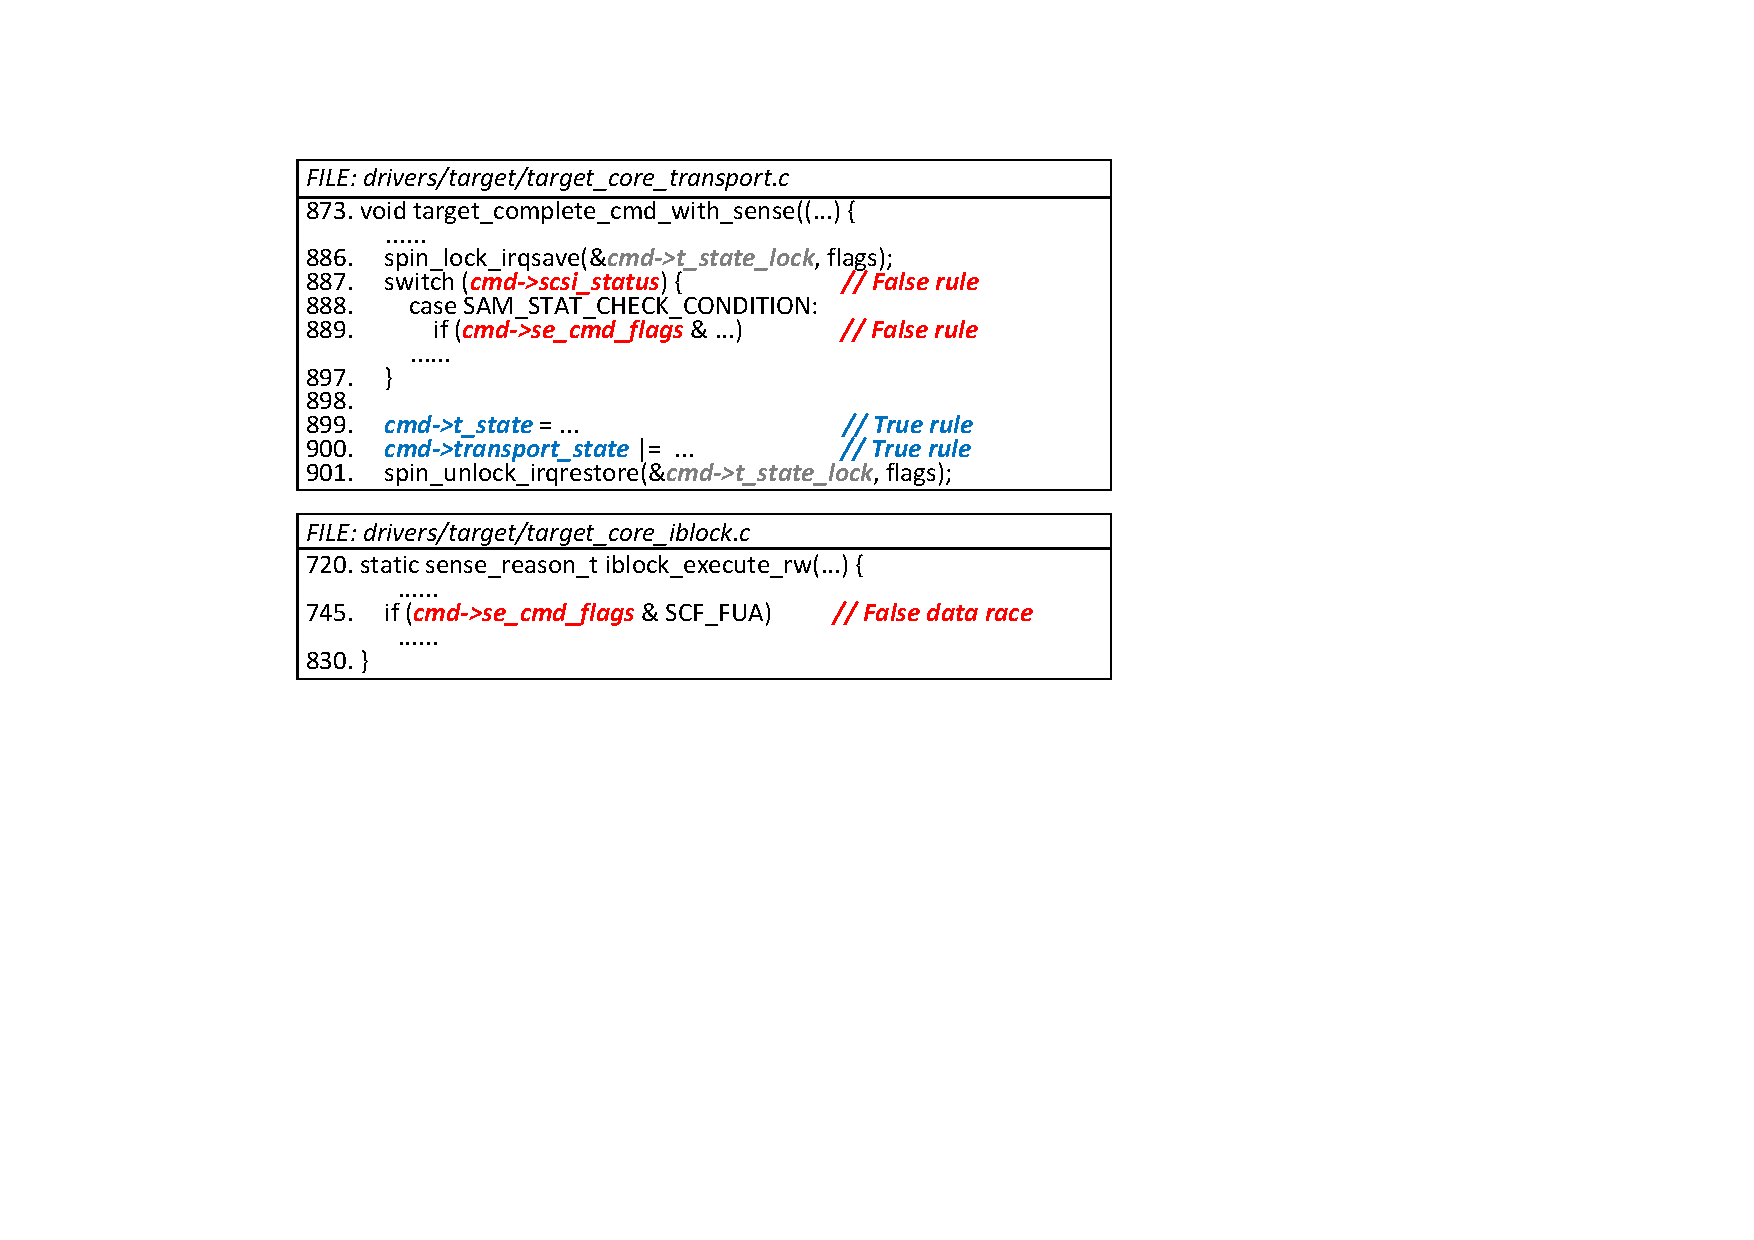
\includegraphics[width=1\linewidth]{figures/fig_demo_false_rule.pdf}
	\figcaption{A false data race caused by an incorrect locking rule.}
	\label{fig_demo_false_rule}
\end{figure}

Figure~\ref{fig_demo_false_rule} shows a false data race caused by an incorrect 
locking rule. In this example, only accesses to {\em cmd->t\_state} and {\em 
cmd->transport\_state} should be protected by the lock {\em 
cmd->t\_state\_lock}. However, the lock operation is put ahead of the switch 
statement by developers, making our alias-aware rule mining method deduce that 
{\em cmd->scsi\_status} and {\em cmd->se\_cmd\_flags} also need to be protected 
by {\em cmd->t\_state\_lock} mistakenly. Based on this incorrect locking rule, 
\sys reports a false positive at Line 745 when {\em cmd->se\_cmd\_flags} is 
accessed in an if statement. Although this data race is a false positive, it 
can cause performance degradation because the critical zone protected by the 
lock/unlock pair should have been limited to Lines 899-900.

Second, in order to reduce memory overhead and improve the performance of data 
passing among different functions, an integer can be divided into several bit 
vectors to represent different data structure fields. However, in the LLVM 
bytecode, accesses to these vectors are divided into a load operation and 
several bit operations, and thus \sys can not distinguish accesses to different 
fields and reports false data races, because not all these fields should be 
protected by a lock. This reason causes \sys to report 14 false data races.

Apart from false data races caused by the two main reasons, there are still 7 
other data races. \sys regards functions without caller functions in a kernel 
module as the entry functions and starts analysis from these entries. However, 
in 4 cases, an assertion is put at the beginning of the entry function, to 
guarantee that the required lock is held, but \sys does not consider assertions 
and the subsequent accesses are regarded as unprotected. The other 3 false data 
races are accessed with {\em READ\_ONCE} or {\em WRITE\_ONCE}, and can not 
cause serious issues.

\PP{False negatives.} \sys may still miss some real data races for three main 
reasons:

First, our alias-aware mining method only considers accessed variables and 
protecting locks that exist in the same data structure. However, on the one 
hand, some accesses to variables may be protected by a global lock in a module, 
and this lock is used to protect accesses to various variables and does 
not exist in any data structure. On the other hand, some special lock 
-acquiring/release functions (such as {\em rcu\_read\_lock} and {\em 
rcu\_read\_unlock}) do not have an argument and are not handled in an alias 
graph. Therefore, locking rules in the above two cases can be missed by our 
alias-aware mining method. As a result, data races that violate these locking 
rules can not be detected by \sys.

Second, \sys does not handle function-pointer calls, and thus it can not build 
complete call graphs for inter-procedural analysis. However, \sys starts 
from functions without caller functions and performs analysis along call 
graphs. And as a result, functions that are only called indirectly through 
function pointers can not be analyzed by \sys, and thus data races involving 
code reached through function-pointer calls can be missed.

Finally, \sys exploits a lock-usage analysis to filter out false data races 
caused by code that can not execute concurrently. Specifically, the lock-usage 
analysis extracts all functions that are reachable from the lock initialization 
functions in a call graph with the union-find set, and assumes that these 
functions can not execute concurrently. However, A function can be called under 
different calling contexts, and some of the calling contexts do not contain 
lock initialization operations, but data races that exist in these functions 
are all dropped by our lock-usage analysis, if any calling context contains a 
lock initialization operation.

\subsection{Case Studies of the Found Harmful Data Races}
\label{subsec_case_study}

Figure~\ref{fig_case_bugs} shows three data races found by \sys in Linux 6.2,
and they have been confirmed by Linux kernel developers.

\begin{figure*}[htbp]
	\centering
	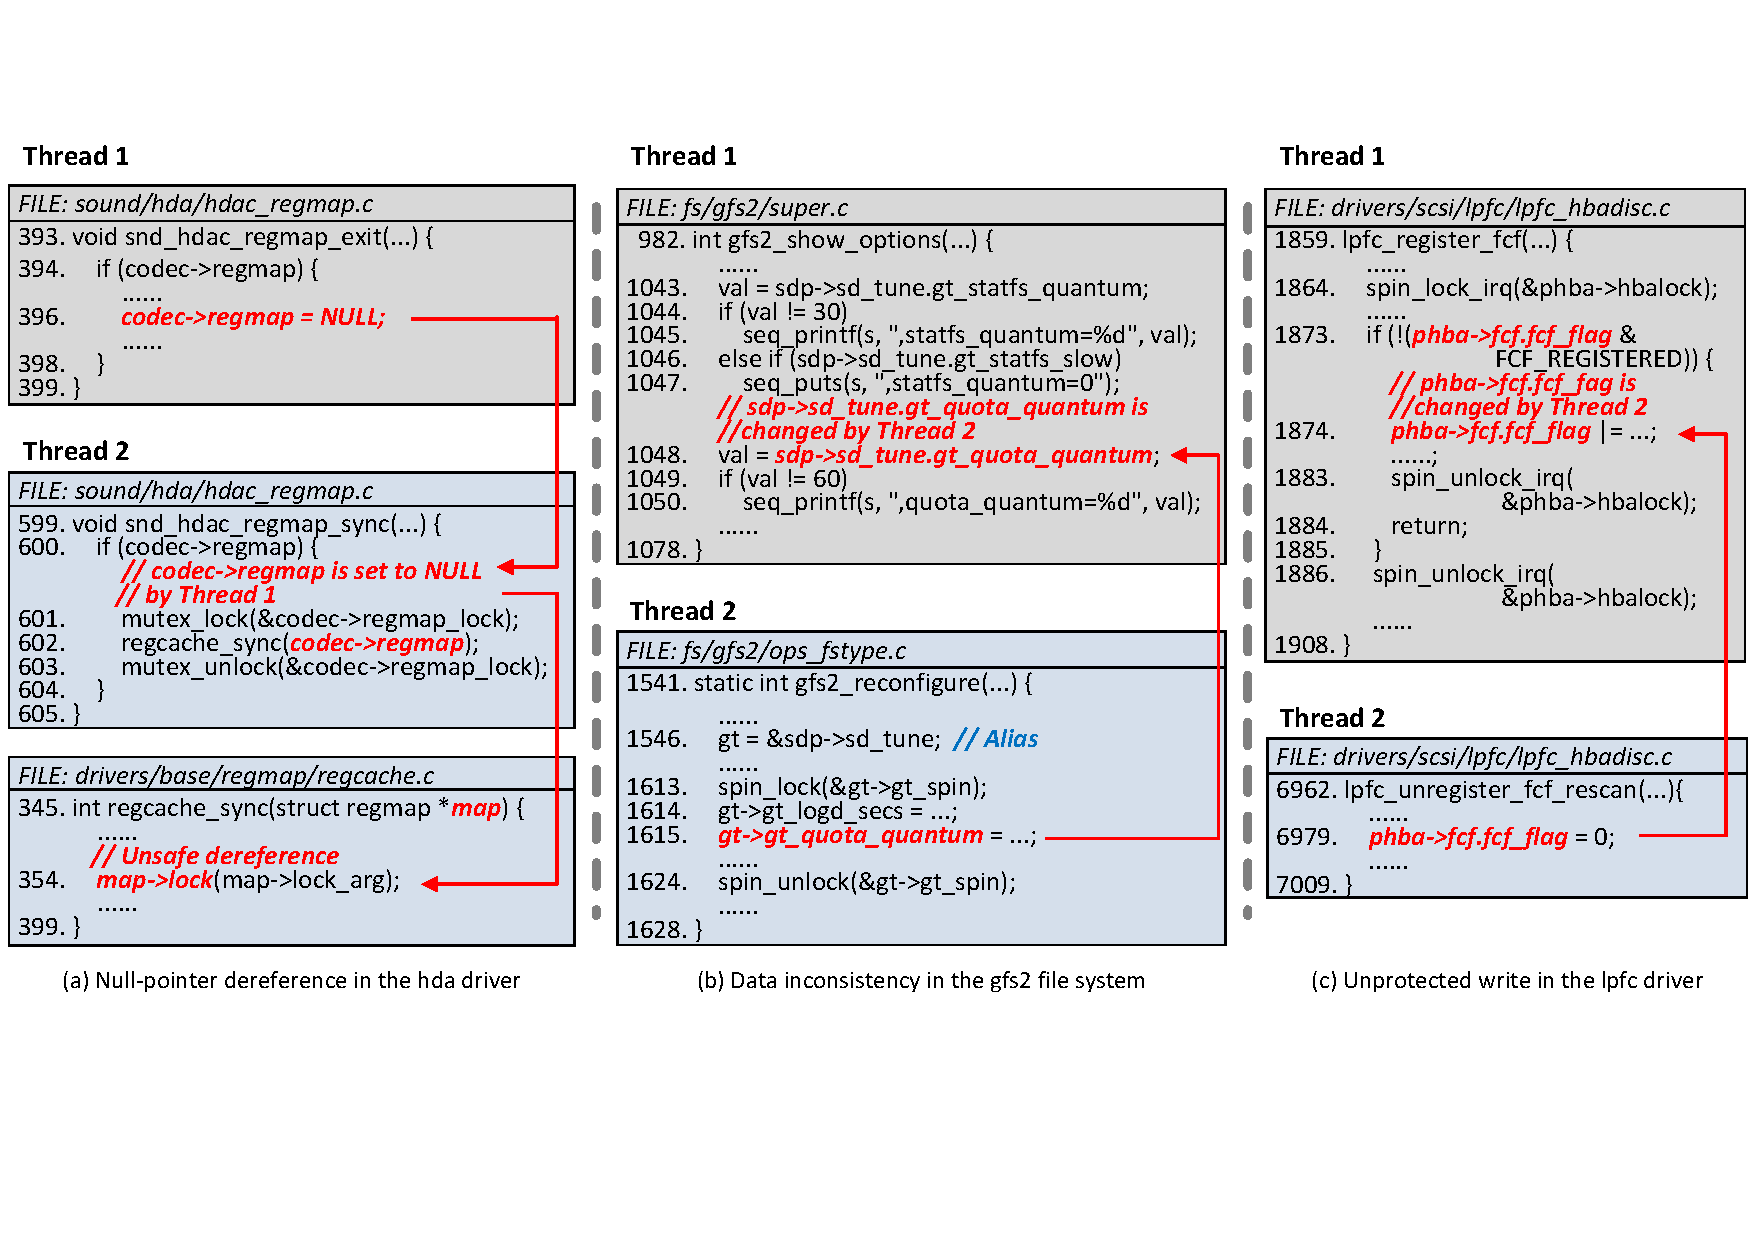
\includegraphics[width=1\linewidth]{figures/fig_case_bugs.pdf}
	\figcaption{Three real data races found by \sys in Linux 6.2.}
	\label{fig_case_bugs}
\end{figure*}

\PP{Null-pointer dereference in the HDA sound driver.} In 
Figure~\ref{fig_case_bugs}(a), the functions {\em snd\_hdac\_regmap\_exit()} 
and {\em snd\_hdac\_regmap\_sync()} can execute concurrently. In Thread 2, the 
variable {\em codec->regmap} is checked by an if statement in the function {\em 
snd\_hdac\_regmap\_sync()}. Right after the condition of the if statement is 
calculated to be true, the variable {\em codec->regmap} is set to NULL by the 
function {\em snd\_hdac\_regmap\_exit()} in Thread 1. And then the function 
{\em regcache\_sync()} is called in Thread 2, with the argument {\em 
codec->regmap}, after acquiring the lock {\em codec->regmap\_lock}. In the 
called function, the variable {\em codec->regmap} is dereferenced through 
{\em map->lock()}. In this execution case, the data structure field {\em 
codec->regmap} is first assigned with NULL in Thread 1, and then dereferenced 
in Thread 2, and thus cause a null-pointer dereference.

\PP{Data inconsistency in the GFS2 file system.} In 
Figure~\ref{fig_case_bugs}(b), the functions {\em gfs2\_show\_options()} and 
{\em gfs2\_reconfigure()} can execute concurrently. In Thread 1, several fields 
such as {\em gt\_statfs\_quantum} and {\em gt\_quota\_quantum} of {\em 
sdp->sd\_tune} are accessed and their values are printed to logs. However, if 
the value of {\em gt->gt\_quota\_quantum} is updated by the function {\em 
gfs2\_reconfigure()} in Thread 2 right before the access to it in Thread 1, the 
values of different fields recorded in logs can be inconsistent.

\PP{Double fetch in the LPFC SCSI driver.} In Figure~\ref{fig_case_bugs}(c), 
the value of the shared variable {\em phba->fcf.fcf\_flag} is set to 0 by the 
function {\em lpfc\_unregister\_fcf\_rescan()} in Thread 2, without acquiring 
the lock {\em phba->hbalock}, and this can cause double fetches in several 
program sites, even if other accesses are all protected by a lock. For example, 
if {\em phba->fcf.fcf\_flag} is set to 0 by Thread 2 between the two accesses 
to it in the function {\em lpfc\_register\_fcf()} in Thread 1 (Lines 1873 and 
1874), the values of the two accesses can be different, causing unpredictable 
behaviors.

